Web2py é um \emph{framework open source}, criado por Massimo Di Pierro, escrito e programável em Python, que possui como principal objetivo o desenvolvimento ágil de aplicações web seguras baseadas em bancos de dados \cite{Pierro:Livro}. O foco do Web2py consiste em permitir que o desenvolvedor concentre-se apenas na aplicação que está desenvolvendo, considerando o provimento de três pilares, que são a simplicidade, o desenvolvimento veloz e a segurança \cite{Duarte:Web2py}.

Por simplicidade no contexto do Web2py, prentende-se reduzir a curva de aprendizagem e tempo para desenvolvimento e/ou manutenção. Por isso, o Web2py é considerado um framework \textit{full-stack} sem dependências, ou seja, ele não necessita de instalação e configuração de arquivos ou outros programas. Ele já é disponibilizado de maneira pronta para o desenvolvimento e com todos os seus módulos funcionando, incluindo o servidor web (Rocket WSGI Web Server), banco de dados (por padrão SQLite) e a IDE web (acessível pelo seu navegador) que fornece acesso a todas as principais funcionalidades \cite{Pierro:Livro}.

O segundo pilar, desenvolvimento veloz, é instanciando no Web2py por meio da existência de comportamentos padrões. O programador deve sobrescrevê-los apenas se necessário. Assim, quando os modelos de dados são especificados, tem-se acesso a um painel web de administração do banco de dados, formulários automáticos, dentre outros. Há que se mencionar ainda a facilidade na exportação de dados, disponibilizados em XML, JSON, dentre outros, e também o fornecimento de \emph{wdigets} de alto nível, permitindo a construção ágil de aplicações web relativamente complexas \cite{Gordon:Web2pycookbook}.

Quando se fala em segurança, pode-se destacar a camada de abstração do banco de dados do Web2py, conhecida com DAL (\textit{Database Abstraction Layer}), que elimina a possibilidade de \textit{SQL Injection}. A linguagem para templates previne contra \textit{Cross Site Scripting}. Os formulários gerados pelo Web2py fornecem validação e bloqueiam a ameaça de \textit{Cross Site Request Forgeries}. Senhas são sempre armazenadas como \textit{hashes}.  Sessões são armazenadas por padrão apenas no servidor, afim de prevenir \textit{Cookie Tampering} e cookies de sessões possuem  identificadores únicos e próprios visando previnir roubos \cite{Pierro:Livro}.

A simplicidade e o desenvolvimento veloz podem ser consideradas as principais justificativas da adoção do framework Web2py como plataforma de desenvolvimento deste trabalho. Menciona-se também a utilização da linguagem de programação Python; a fácil aprendizagem dos conceitos relativos a este \emph{framework}, justificado pelo cronograma de desenvolvimento relativamente curto; e também aspectos de caráter mais técnico e tecnológico, como a possibilidade de integração com diferentes bancos de dados \emph{open source}, a utilização de tecnologias como Bootstrap e jQuery e o fato do Web2py seguir o padrão arquitetural MVC, que permite uma melhor organização do código.

\subsection{Padrão de Projeto MVC}

O MVC (do inglês, \emph{Model-View-Controller}) é o padrão de projeto mais popularmente adotado pelos \emph{frameworks} de desenvolvimento de aplicações web. Este padrão de projeto incentiva o desenvolvedor a separar as camadas de negócio(\emph{Model}) e de apresentação dos dados (\emph{View}), por meio da inclusão de uma camada de controle de fluxo de trabalho(\emph{Controller}), que atua como uma camada intermediária\cite{Pierro:Livro}. Uma visão geral do padrão MVC é ilustrada na Figura \ref{fig:padraomvc}.

\begin{figure}[H]
	\centering
	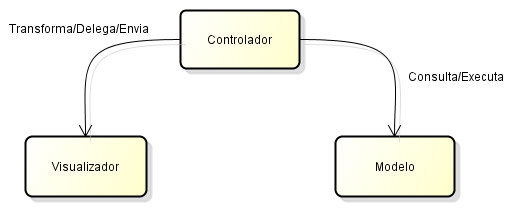
\includegraphics[width=0.6\textwidth]{./img/mvc.png}
	\caption{Visão geral do padrão de projeto MVC. Fonte: \cite{Weissman:MVC} \label{fig:padraomvc}}
\end{figure}

O \textit{modelo} diz respeito à toda a parte do sistema responsável pela lógica de negócio e seus componentes auxiliares, como persistência, criação das tabelas de banco de dados, definição das classes utilizadas na aplicação, etc. O \textit{visualizador}, por sua vez, é a parte visível ao usuário final. No caso das aplicações web, é a página HTML resultante desta camada. Por fim, o \emph{controlador} sincroniza a interação entre as duas camadas anteriores.Por exemplo, quando o usuário clica em um \textit{link} da página HTML exibida, o controlador é acionado e transforma os parâmetros de entrada (String geralmente) para um formato compatível com a camada de negócio (inteiros, doubles, objetos de classes, etc), cujo resultado do  processamento é recebido pelo controlador, que o modifica, caso necessário, e em seguida o envia à camada de visualização para que seja apresentado ao usuário final \cite{Weissman:MVC}.

O Web2py adota em seu processo de desenvolvimento o MVC como padrão de projeto, e isso pode ser facilmente percebido visualizando a estrutura de diretórios criada pelo framework, visando assim, facilitar o gerenciamento de projetos a serem desenvolvidos, proporcionando ganhos de manutenibilidade, pois o desenvolvedor precisa lidar com menos dependências \cite{Pierro:Livro}.
